% !TEX encoding = UTF-8 Unicode

%=============================================
%---(C) QESOFT, Isabel Sampaio (ais@isep.ipp.pt), 2019 ---
%=============================================

%----------tipo de documento------------------
\documentclass[openany,10pt,a4paper]{article}

% ----------------------
% Configuração página

\usepackage
[
a4paper,
left=2.6cm,
right=2.4cm,
top= 2.6 cm,
bottom=1.5 cm,
]
{geometry}


% ---- Sem indentação parágrafo -------
\setlength\parindent{0pt} 
\setlength{\voffset}{-0.2in}

% ---- Espaçamento entre parágrafos -------
\setlength{\parskip}{5pt}

% -----Topo------------------
\setlength{\topmargin}{-\headheight}
\setlength{\headsep}{0.0cm}

% -----Espaçamento palavras---------------
\renewcommand{\baselinestretch}{1.0}   

%------ Tabelas -----
\usepackage{longtable}

% ------------------ Opções em tabelas-----------------
\usepackage{array}		% para centrar colunas (de tabelas) com p{XXcm}
\usepackage{paralist}	% para colocar enumerates em linha com um parágrafo

\usepackage{booktabs,multirow} 
\usepackage{longtable}
\usepackage{tabularx}
\usepackage{subcaption}
\usepackage{longtable}
\usepackage{xcolor}
\usepackage{tabu}
\usepackage{tabulary}
\usepackage{float}

% -----------------PORTUGUES----------
\usepackage[utf8]{inputenc}
\usepackage[T1]{fontenc}

%-----tipo letra---------
\usepackage{helvet} % --- não existe Calibri em  pdflatex
\renewcommand{\familydefault}{\sfdefault}

%---Portuguese-specific commands ----
\usepackage[english,portuguese]{babel}
 
% -----------------   Hyphenation rules ----------------
\usepackage{hyphenat}
\hyphenation{re-cu-pe-rar te-ma ma-té-ri-a ci-en-tí-fi-co}

%-------------------------------------------------------------------------------------------------------
%para palavras que ao quebrar leva 2 hifen ,: por exemplo "verificou-se": no texto fazer verificou{-}{-}se
\defineshorthand{"-}{\nobreak\hskip0pt\discretionary{-}{-}{-}\nobreak\hskip0pt} 

% ---------- Hyperlinks ------------
\usepackage{cooltooltips} 
\def\cool{\texttt{cool}}

\usepackage{verbatim}

% -------- Incluir pdfs-------
\usepackage{graphicx}
\graphicspath{ {./images/} }

%---------Para Titulos: capitulos, secções, etc.-----------
\usepackage{titlesec}

\titleformat{\section} {\Large\bfseries}{\thesection.}{1em}{}
\titleformat*{\subsection}{\large}
\titleformat*{\subsubsection}{\large}

%------------- espaçamento antes/depois titulos -----------

\titlespacing{\section}{0pt}{*1.1}{*1.0}
\titlespacing{\subsection}{0pt}{*1.1}{*1.0}
\titlespacing{\subsubsection}{0pt}{*1.1}{*1.0}

 %--------- Inicio do documento--------------------
\begin{document}
\pagenumbering{arabic}

\title{\textbf{Uma visão sobre a Qualidade de Processo e de Produto em ambiente académico}}
\author{João Cardoso, \textit{1150943} \\ Sofia Silva, \textit{1150690} \\ Tiago Leite, \textit{1150780}}
\date{}

\maketitle

% -------------- SECÇÕES ---------------
\section{Introdução}
Este trabalho foi realizado no âmbito da unidade curricular de Qualidade na Engenharia de Software com o objetivo de avaliar a qualidade do software de um projeto desenvolvido. A avaliação realizada foi dividida em duas partes, a avaliação do processo, usando o modelo CMMI e a avaliação do produto, usando o modelo OMG.

\section{Escolha do Projecto}
O projeto escolhido para ser avaliado na vertente do processo e produto é o projeto Cleansheets. Este projeto foi realizado no ano letivo de 2015/2016 no âmbito da Unidade de Curricular de Laboratório/Projeto IV da Licenciatura em Engenharia Informática e tinha como objetivo desenvolver uma aplicação de folhas de cálculo com funcionalidades avançadas – tais como cooperação remota, formatação de texto avançada e suporte para macros e fórmulas – de forma a poderem ser aplicadas boas práticas de desenvolvimento e metodologias ágeis de organização de trabalho.\\
A escolha deste projeto prende-se ao facto de ser um projeto cujo âmbito, arquitetura e funcionamento é conhecido por todos os membros do grupo, facilitando assim o processo de análise de processo e de produto. 

\section{Análise do projeto}
Nesta secção estão presentes as duas análises de qualidade realizadas ao projeto escolhido. Primeiramente a análise ao processo e posteriormente a análise ao produto.

\subsection{Análise da Qualidade do Processo}
Nesta subsecção é apresentada, tal como pedido, uma análise informal ao processo utilizado no decorrer do projeto escolhido (LAPR4). Enquadra-se primeiramente o conceito de qualidade de processo e um exemplo da sua aplicação num caso real com recurso ao CMMI For Development. \\
Os modelos CMMI(\textit{Capability Maturity Model Integration}), desenvolvidos por equipas multidisciplinares da Universidade de Carnegie Mellon, incluindo o SEI (\textit{Software Engineering Institute}), são coleções de boas práticas que procuram ajudar as organizações a melhorar os seus processos. O modelo CMMI-DEV (CMMI for Development) é especialmente ligado aos processos de desenvolvimento de produtos e serviços, daí a sua utilização no meio do desenvolvolvimento de software. Este possui orientações com foco na melhoria da qualidade final do produto para cumprir as necessidades dos consumidores finais \cite{CMMIProductTeam2010}.\\ 
A análise da qualidade de processo a seguir apresentada teve como base uma representação discreta com foco nos níveis 2 e 3 de maturidade e em 7 e 11 áreas de processo para cada um desses níveis respetivamente. Para a obtenção de resultados foi elaborado um questionário (em anexo) com um conjunto questões para cada uma das áreas de processo, estando dessa forma dividido. Para cada um dos processos existem 4 possíveis respostas: Totalmente Implementado, Implementado Parcialmente, Não Implementado ou Não Sei caso não seja aplicável ou seja desconhecido.

\subsubsection{Resultados}
Nesta subsecção são apresentados os resultados relativos ao questionário desenvolvido, presente no Anexo \ref{anexo_processo}. \\
De forma a facilitar a análise dos resultados, foi organizado o resumo para cada área de processo, apresentando o seu objetivo, as metas definidas, assim como as respetivas avaliações seguindo os critérios definidos no Anexo \ref{anexo_processo_classificacao}.

\textbf{Gestão de Configuração: Não Satisfeita} \\
\textbf{- Objetivo:} Permitir a integração contínua dos vários componentes de software em que as mudanças são devidamente documentadas. \\ \\
\begin{tabular}{|p{3.7in}|p{1in}|p{1in}|}
	\hline
	\textbf{Meta} & \textbf{Questões} & \textbf{Avaliação} \\ \hline
	Identificar e definir as configurações disponíveis & 1 e 2 & NSat \\
	Monitorizar as alterações de configuração  & 3 e 4 & NSat \\
	Documentar as alterações de configuração  & 5, 6 e 7 & NSat \\ \hline
\end{tabular} \\

\textbf{Medição e Análise: Não Satisfeita} \\ 
\textbf{- Objetivo:} Permitir à organização realizar uma medição da sua qualidade. \\ \\
\begin{tabular}{|p{3.7in}|p{1in}|p{1in}|}	 \hline
\textbf{Meta} & \textbf{Questões} & \textbf{Avaliação} \\ \hline
Definir mecanismos de medição & 8, 9, 10, 11 & NSat \\
Pôr em prática os mecanismos definidos  & 12, 13 & NSat \\
Os mecanismos são utilizados ativamente na organização & 14 e 15 & NSat \\ \hline
\end{tabular} \\

\textbf{Monitorização e Controlo do Projeto: Não Satisfeita} \\ 
\textbf{- Objetivo:} Permitir à organização uma monitorização do progresso dos projetos em curso. \\
\\
\begin{tabular}{|p{3.7in}|p{1in}|p{1in}|}	\hline
\textbf{Meta} & \textbf{Questões} & \textbf{Avaliação} \\ \hline
Criar métricas de monitorização de progresso de projetos em relação ao planeado & 17, 18, 19 e 20 & NSat \\
Utilizar o controlo do progresso dos projetos para organizar retrospetivas & 16, 21, 22, 23 & NSat \\
Aplicar efetivamente medidas corretivas para os processos negativamente identificados na monitorização & 24 e 25 & NSat \\\hline
\end{tabular} \\

\textbf{Planeamento de Projeto: Não Satisfeita} \\ 
\textbf{- Objetivo:} Melhorar a fase de planeamento de projetos da organização. \\
\\
\begin{tabular}{|p{3.7in}|p{1in}|p{1in}|}\hline
\textbf{Meta} & \textbf{Questões} & \textbf{Avaliação} \\ \hline
Definir a estrutura de estimativa do planeamento & 26 e 27 & NSat \\
As estimativas são eficazes e mantidas ao longo do projeto & 29 e 30 & NSat \\
Toda a estrutura definida para o planeamento é identificada, analisada e monitorizada & 31, 32, 33, 34, 35 e 36 & NSat \\ 
Há uma revisão e apoio à execução do planeamento efetuado & 37, 38 e 39 & NSat \\ \hline
\end{tabular} 

\textbf{Garantia da Qualidade de Processo e Produto: Não Satisfeita} \\
\textbf{- Objetivo:} Registar e monitorizar a qualidade do processo e produto \\
\\
\begin{tabular}{|p{3.7in}|p{1in}|p{1in}|}	\hline
\textbf{Meta} & \textbf{Questões} & \textbf{Avaliação} \\ \hline
Avaliar e definir os registos de atividades de qualidade & 40 e 41 & NSat \\ 
Manter e cumprir os registos definidos & 42 e 43 & NSat \\ \hline
\end{tabular}

\textbf{Gestão de Requisitos: Satisfeita} \\
\textbf{- Objetivo:} Estabelecer o sincronismo entre os requisitos e o desenvolvimento \\
\\
\begin{tabular}{|p{3.7in}|p{1in}|p{1in}|}	\hline	
\textbf{Meta} & \textbf{Questões} & \textbf{Avaliação} \\ \hline
Manter o compromisso e comunicação entre gestores de requisitos desenvolvedores & 44, 45, 46, 47 e 48 & Sat \\ \hline
\end{tabular}

\textbf{Gestão de Contrato com Fornecedores: Não Aplicável} \\ 
\textbf{- Objetivo:} Estabelecer contacto com os fornecedores e controlo do processo de fornecimento \\
\\
\begin{tabular}{|p{3.7in}|p{1in}|p{1in}|}	\hline
\textbf{Meta} & \textbf{Questões} & \textbf{Avaliação} \\ \hline
Escolher os melhores fornecedores e os recursos realmente necessários ao projeto & 49 e 50 & NAv \\ 
Manter o contacto com o fornecimento e assegurar o seu cumprimento & 51, 52, 53 e 54 & NAv \\ \hline
\end{tabular}

\textbf{Análise e Tomada de Decisões: Não Satisfeita} \\  
\textbf{- Objetivo:} Criar métodos que melhorem o rigor da análise e tomada de decisões \\
\\
\begin{tabular}{|p{3.7in}|p{1in}|p{1in}|} \hline	
\textbf{Meta} & \textbf{Questões} & \textbf{Avaliação} \\ \hline
Definir métodos de avaliação e de análise & 55, 56, 57 e 58 & NSat \\ 
Manter o cumprimento dos procedimentos de análise e decisão & 59 e 60 & NSat \\ \hline
\end{tabular}

\textbf{Gestão Integrada do Projeto: Não Satisfeita} \\ 
\textbf{- Objetivo:} Definir os processos desejados para o desenvolvimento e assegurar que são seguidos \\
\\
\begin{tabular}{|p{3.7in}|p{1in}|p{1in}|}	\hline
\textbf{Meta} & \textbf{Questões} & \textbf{Avaliação} \\ \hline
Definir processos de desenvolvimento & 61, 63, 64 e 66 & NSat \\
Verificar que o processo está a ser assegurado e reajustar se for necessário & 62, 65, 67, 68, 69 e 70 & NSat \\ \hline
\end{tabular}

\textbf{Definição dos Processos da Organização: Não Satisfeita} \\
\textbf{- Objetivo:} Estabelecer os processos da organização \\
\\
\begin{tabular}{|p{3.7in}|p{1in}|p{1in}|}	\hline	
\textbf{Meta} & \textbf{Questões} & \textbf{Avaliação} \\ \hline
Estabelecer e manter os processos e critérios padrão da organização & 71, 72, 73, 74, 75, 76 e 77 & NSat \\ \hline
\end{tabular}

\textbf{Enfoque nos Processos da Organização: Não Satisfeita} \\ 
\textbf{- Objetivo:} Procurar melhorar os processos da organização \\
\\
\begin{tabular}{|p{3.7in}|p{1in}|p{1in}|}	\hline	
\textbf{Meta} & \textbf{Questões} & \textbf{Avaliação} \\ \hline
Controlar periodicamente os processos da organização em termos de qualidade & 78, 79, 80, 85 e 86 & NSat \\
Encontrar e implementar as ações de melhoria encontradas pelo controlo & 81, 82, 83 e 84 & NAv \\ \hline
\end{tabular}

\textbf{Formação na Organização: Não Satisfeita} \\ 
\textbf{- Objetivo:} Formar de forma rentável os membros da organização \\
\\
\begin{tabular}{|p{3.7in}|p{1in}|p{1in}|}		\hline
\textbf{Meta} & \textbf{Questões} & \textbf{Avaliação} \\ \hline
Encontrar necessidades de formação e determinar a melhor forma de as colmatar & 87, 88, 89, 90 e 91 & NAv \\
Elaborar, implementar e avaliar um plano de formações & 92 e 93 & NSat \\ \hline
\end{tabular}

\textbf{Integração de Produto:  Não Satisfeita} \\ 
\textbf{- Objetivo:} Manter a integridade e expansibilidade do produto \\
\\
\begin{tabular}{|p{3.7in}|p{1in}|p{1in}|}		\hline
\textbf{Meta} & \textbf{Questões} & \textbf{Avaliação} \\ \hline
Elaborar diretrizes de desenvolvimento sustentável & 94, 95, 96, 98 & NSat \\
Desenvolver revisões ao estado de integração dos componentes do produto & 97, 99, 100, 101 e 102 & NSat \\ \hline
\end{tabular}

\textbf{Desenvolvimento de Requisitos: Não Satisfeita} \\ 
\textbf{- Objetivo:} Desenvolver o produto requisitado pelo cliente \\
\\
\begin{tabular}{|p{3.7in}|p{1in}|p{1in}|}	\hline
\textbf{Meta} & \textbf{Questões} & \textbf{Avaliação} \\ \hline
Efetuar um levantamento e análise de requisitos frequente & 103, 104, 105, 106, 107, 108, 109, 110, 111 e 112 & NSat \\ \hline
\end{tabular}

\textbf{Gestão de Risco: Não Satisfeita} \\ 
\textbf{- Objetivo:} Identificar os riscos inerentes a cada componente do produto em desenvolvimento e assim definir a sua prioridade \\
\\
\begin{tabular}{|p{3.7in}|p{1in}|p{1in}|}		 \hline
\textbf{Meta} & \textbf{Questões} & \textbf{Avaliação} \\ \hline
Definir critérios de avaliação de risco & 113, 114, 115 e 116 & NSat \\
Aplicar os critérios de risco para avaliações periódicas e levantamento de prioridades & 117, 118 e 119 & NSat \\ \hline
\end{tabular}

\textbf{Solução Técnica: Não Satisfeita} \\ 
\textbf{- Objetivo:} Criar documentação técnica para as soluções e procurar alternativas \\
\\
\begin{tabular}{|p{3.7in}|p{1in}|p{1in}|} \hline		
\textbf{Meta} & \textbf{Questões} & \textbf{Avaliação} \\ \hline
Procurar e escolher melhores alternativas para resolução de problemas & 120, 121, 124, 125 & NSat \\
Documentar as soluções de software desenvolvidas & 122, 123, 126 e 127 & NSat \\ \hline
\end{tabular}

\textbf{Validação: Não Satisfeita} \\ 
\textbf{- Objetivo:} Planear e assegurar a utilização de mecanismos de validação do produto desenvolvido \\
\\
\begin{tabular}{|p{3.7in}|p{1in}|p{1in}|}	\hline	
\textbf{Meta} & \textbf{Questões} & \textbf{Avaliação} \\ \hline
Criar plano de validação de produto & 128 e 130 & NSat \\
Assegurar a realização da validação dos produtos e analisar os seus resultados & 129, 130, 131 e 132 & NSat \\ \hline
\end{tabular}

\textbf{Verificação: Não Satisfeita} \\ 
\textbf{- Objetivo:} Planear e assegurar a utilização de mecanismos de verificação do produto desenvolvido \\
\\
\begin{tabular}{|p{3.7in}|p{1in}|p{1in}|}		\hline
\textbf{Meta} & \textbf{Questões} & \textbf{Avaliação} \\ \hline
Criar plano de verificação de produto & 133, 135 e 136 & NSat \\
Assegurar a realização da verificação dos produtos e analisar os seus resultados & 134, 137, 138, 139 e 140 & NSat \\ \hline
\end{tabular}

\subsection{Qualidade do Produto}
A avaliação do modelo de qualidade do produto pode ser elaborada avaliando recorrendo a um conjunto de características contempladas no modelo de qualidade ISSO/IEC 25000, descritas na figura ~\ref{fig_quality}. A avaliação descrita neste documento assentará-se nas características de Manutenibilidade, Segurança, Eficiência de Performance e Fiabilidade.

\begin{figure}[h]
	\centering
	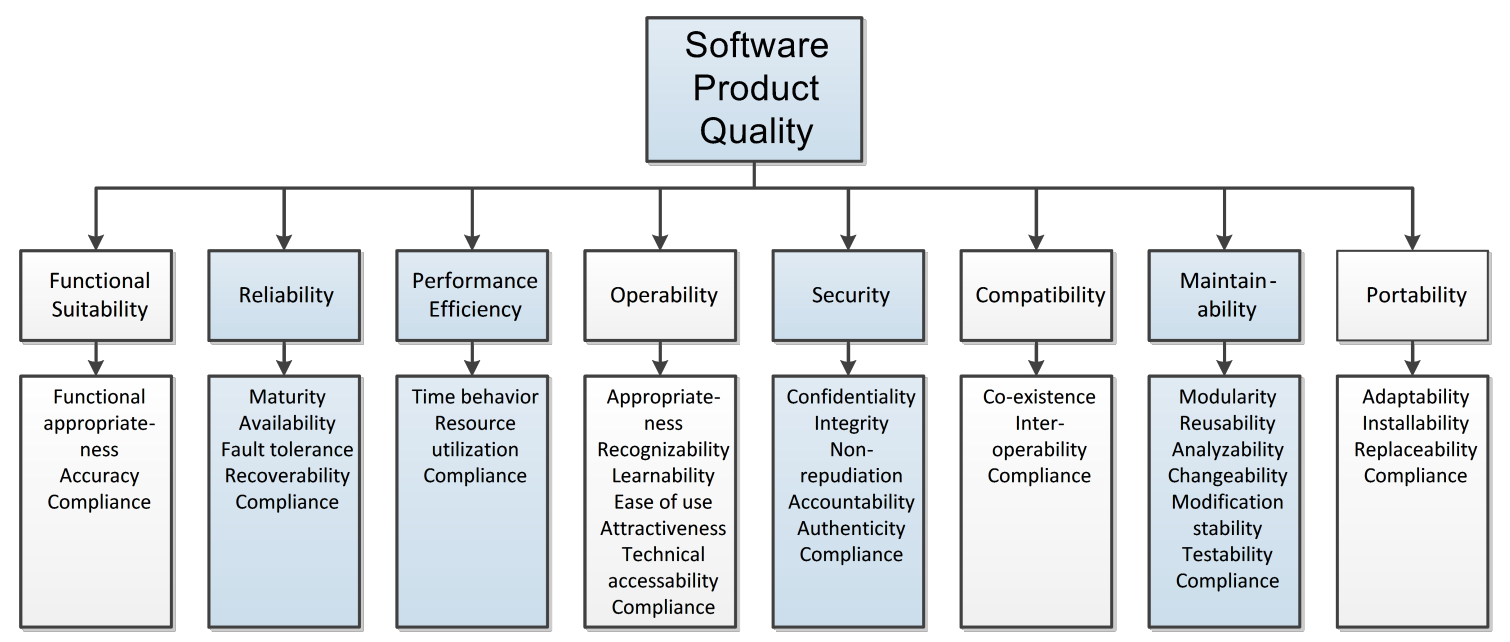
\includegraphics[width=1\linewidth]{quality.PNG}
	\caption{Caraterísticas da qualidade de software de acordo com a norma ISO/IEC 25010 \small{\textit{Fonte: 	\cite{OMG_Performance}}}}
	\label{fig_quality}
\end{figure}

Definiu-se o questionário presente no anexo ~\ref{anexo_produto}, baseado na especificação definida nos padrões da Object Management Group (OMG) para proceder à avaliação. \\
Uma vez que o projeto escolhido para a análise contém 793 classes de código desenvolvido na linguagem Java, foi aplicada 
\textit{Hubbard’s Rule of Five}, selecionando 5 classes aleatórias para contabilizar o número de ocorrências de cada métrica definida no questionário. As classes selecionadas foram BeanShellLoader (C1), HandlerUserChatDTO (C2), PdfExport (C3), ThreadExport (C4) e UnlinkExportDataAction (C5).

\subsubsection{Manutenibilidade}
Esta caraterística contabiliza o número de violações de boas práticas arquiteturais que fazem com que o software desenvolvido seja difícil de ser modificado, aumentando o esforço exigido no seu suporte e na sua adaptação a novos requisitos. Estas violações podem resultar em operações não confiáveis, tais como interrupções, corrupção de dados e longa recuperação de falhas do sistema. \cite{OMG_Maintainability}

	\begin{longtable}{|p{1.2in}|p{0.28in}|p{0.28in}|p{0.28in}|p{0.28in}|p{0.28in}|p{0.35in}|}
		\caption{Número de violações em cada classe por regra de manutenibilidade}
		\label{table_manutenibilidade}
		\endhead
		\hline
		\textbf{Regra} & \textbf{C1} & \textbf{C2} & \textbf{C3} & \textbf{C4} & \textbf{C5} & \textbf{Final} \\ \hline
		ASCMM-MNT-1 & 0 & 0 & 0 & 0 & 0 & 0 \\ \hline
		ASCMM-MNT-2 & 0 & 2 & 0 & 1 & 0 & 3 \\ \hline
		ASCMM-MNT-3 & 0 & 0 & 0 & 0 & 0 & 0 \\ \hline
		ASCMM-MNT-4 & 0 & 0 & 0 & 0 & 0 & 0 \\ \hline
		ASCMM-MNT-5 & 0 & 0 & 0 & 0 & 0 & 0 \\ \hline
		ASCMM-MNT-6 & 0 & 2 & 0 & 0 & 0 & 2 \\ \hline
		ASCMM-MNT-7 & 0 & 0 & 0 & 0 & 0 & 0 \\ \hline
		ASCMM-MNT-8 & 0 & 0 & 0 & 0 & 0 & 0 \\ \hline
		ASCMM-MNT-9 & 0 & 0 & 0 & 0 & 0 & 0 \\ \hline
		ASCMM-MNT-10 & 0 & 0 & 0 & 0 & 0 & 0 \\ \hline
		ASCMM-MNT-11 & 0 & 0 & 2 & 0 & 0 & 2 \\ \hline
		ASCMM-MNT-12 & 0 & 0 & 0 & 0 & 0 & 0 \\ \hline
		ASCMM-MNT-13 & 0 & 0 & 1 & 0 & 0 & 1 \\ \hline
		ASCMM-MNT-14 & 0 & 0 & 1 & 0 & 0 & 1 \\ \hline
		ASCMM-MNT-15 & 0 & 0 & 4 & 0 & 0 & 4 \\ \hline
		ASCMM-MNT-16 & 0 & 3 & 5 & 4 & 0 & 12 \\ \hline
		ASCMM-MNT-17 & 0 & 0 & 0 & 0 & 0 & 0 \\ \hline
		ASCMM-MNT-18 & 0 & 0 & 1 & 0 & 0 & 1 \\ \hline
		ASCMM-MNT-19 & 0 & 0 & 3 & 0 & 0 & 3 \\ \hline
		ASCMM-MNT-20 & 0 & 0 & 2 & 0 & 2 & 2 \\ \hline
	\end{longtable}
Após a contabilização de violações de cada métrica apresentada na tabela ~\ref{table_manutenibilidade}, seguiu-se o calculo da medida base de manutenibilidade. Para obter este valor, é necessário realizar o somatório de todas as violações detetadas, chegando assim ao valor 31.
$$\sum_{n=1}^{20} CISQ - MntME_{20} = 31$$

\subsubsection{Segurança}
Esta caraterística contabiliza o número de violações de boas práticas arquiteturais que fazem com que o software permita a entrada não autorizada em sistemas, roubo de informações confidenciais, entre outros \cite{OMG_Security}. A partir desta medida é possível saber o grau de proteção que o sistema tem, para que pessoas e/ou outros produtos ou sistemas tenham o grau de acesso aos dados adequado aos seus tipos e níveis de autorização \cite{security_iso}.
\begin{samepage}
\begin{longtable}{|p{1.9in}|p{0.28in}|p{0.28in}|p{0.28in}|p{0.28in}|p{0.28in}|p{0.35in}|}
		\caption{Regras da caraterística segurança}
		\label{table_security}
		\endhead
		\hline	
		\textbf{Regra} & \textbf{C1} & \textbf{C2} & \textbf{C3} & \textbf{C4} & \textbf{C5} & \textbf{Final} \\ \hline
		ASCMM-CWE-22 & 0 & 0 & 0 & 0 & 0 & 0 \\ \hline
		ASCMM-CWE-78 & 0 & 0 & 0 & 0 & 0 & 0 \\ \hline
		ASCMM-CWE-79 & 0 & 0 & 0 & 0 & 0 & 0 \\ \hline
		ASCMM-CWE-89 & 0 & 0 & 0 & 0 & 0 & 0 \\ \hline
		ASCMM-CWE-99 & 0 & 0 & 0 & 0 & 0 & 0 \\ \hline
		ASCMM-CWE-120 & 0 & 0 & 2 & 0 & 1 & 3 \\ \hline
		ASCMM-CWE-129 & 0 & 0 & 0 & 0 & 0 & 0 \\ \hline
		ASCMM-CWE-134 & 0 & 0 & 0 & 0 & 0 & 0 \\ \hline
		ASCMM-CWE-252-resource & 0 & 0 & 0 & 0 & 0 & 0 \\ \hline
		ASCMM-CWE-327 & 0 & 0 & 0 & 0 & 0 & 0 \\ \hline
		ASCMM-CWE-396 & 0 & 0 & 0 & 1 & 0 & 1 \\ \hline
		ASCMM-CWE-397 & 0 & 0 & 0 & 0 & 0 & 0 \\ \hline
		ASCMM-CWE-434 & 0 & 0 & 0 & 0 & 0 & 0 \\ \hline
		ASCMM-CWE-456 & 1 & 0 & 2 & 0 & 0 & 3 \\ \hline
		ASCMM-CWE-606 & 0 & 0 & 0 & 0 & 0 & 0 \\ \hline
		ASCMM-CWE-667 & 0 & 0 & 0 & 0 & 0 & 0 \\ \hline
		ASCMM-CWE-672 & 0 & 0 & 0 & 0 & 0 & 0 \\ \hline
		ASCMM-CWE-681 & 1 & 0 & 0 & 0 & 0 & 1 \\ \hline
		ASCMM-CWE-772 & 0 & 0 & 0 & 0 & 0 & 0 \\ \hline
		ASCMM-CWE-789 & 0 & 0 & 0 & 0 & 0 & 0 \\ \hline
		ASCMM-CWE-798 & 0 & 0 & 0 & 0 & 0 & 0 \\ \hline
		ASCMM-CWE-835 & 0 & 0 & 0 & 0 & 0 & 0 \\ \hline
\end{longtable}
\end{samepage}
Após a contabilização de violações de cada métrica apresentada na tabela ~\ref{table_security}, seguiu-se o calculo da medida base de segurança. Para obter este valor, é necessário realizar o somatório de todas as violações detetadas, chegando assim ao valor 8.
$$\sum_{n=1}^{22} CISQ - SecME_{22} = 8$$

\subsubsection{Eficiência de Performance}
Esta caraterística contabiliza o número de violações de boas práticas arquiteturais que poderão resultar numa operação ineficiente, como a degradação do desempenho ou uso excessivo de recursos do processador \cite{OMG_Performance}.
\begin{longtable}{|p{1.3in}|p{0.28in}|p{0.28in}|p{0.28in}|p{0.28in}|p{0.28in}|p{0.35in}|}
	\caption{Regras da caraterística eficiencia de performance}
	\label{table_performance}
	\endhead
	\hline	
	\textbf{Regra} & \textbf{C1} & \textbf{C2} & \textbf{C3} & \textbf{C4} & \textbf{C5} & \textbf{Final} \\ \hline
ASCPEM-PRF-1 & 0 & 0 & 0 & 0 & 0 & 0 \\ \hline
ASCPEM-PRF-2 & 1 & 0 & 1 & 0 & 0 & 2 \\ \hline
ASCPEM-PRF-3 & 0 & 0 & 4 & 0 & 0 & 4 \\ \hline
ASCPEM-PRF-4 & 0 & 0 & 0 & 0 & 0 & 0 \\ \hline
ASCPEM-PRF-5 & 0 & 0 & 0 & 0 & 0 & 0 \\ \hline
ASCPEM-PRF-6 & 0 & 0 & 0 & 0 & 0 & 0 \\ \hline
ASCPEM-PRF-7 & 0 & 0 & 0 & 0 & 0 & 0 \\ \hline
ASCPEM-PRF-8 & 0 & 0 & 1 & 0 & 0 & 1 \\ \hline
ASCPEM-PRF-9 & 0 & 0 & 0 & 0 & 0 & 0 \\ \hline
ASCPEM-PRF-10 & 0 & 0 & 0 & 0 & 0 & 0 \\ \hline
ASCPEM-PRF-11 & 0 & 0 & 0 & 0 & 0 & 0 \\ \hline
ASCPEM-PRF-12 & 0 & 0 & 2 & 0 & 0 & 2 \\ \hline
ASCPEM-PRF-13 & 0 & 0 & 0 & 0 & 0 & 0 \\ \hline
ASCPEM-PRF-14 & 0 & 0 & 0 & 0 & 0 & 0 \\ \hline
ASCPEM-PRF-15 & 0 & 0 & 0 & 0 & 0 & 0 \\ \hline
	\end{longtable} 

Após a contabilização de violações de cada métrica apresentada na tabela ~\ref{table_performance}, seguiu-se o calculo da medida base de segurança. Para obter este valor, é necessário realizar o somatório de todas as violações detetadas, chegando assim ao valor 9.
$$\sum_{n=1}^{15} CISQ - PrfME_{15} = 9$$

\subsubsection{Fiabilidade}
Esta caraterística contabiliza o número de violações de boas práticas arquiteturais que poderão resultar em operações não confiáveis, como interrupções, corrupção de dados e recuperação de falhas do sistema \cite{OMG_Reliability}. Quanto mais elevado o número de violações, mais provável é, para um determinado período temporal, que o sistema tenha uma falha. 
\begin{longtable}{|p{1.9in}|p{0.28in}|p{0.28in}|p{0.28in}|p{0.28in}|p{0.28in}|p{0.35in}|}
	\caption{Regras da caraterística fiabilidade}
	\label{table_Reliability}
	\endhead
	\hline	
		\textbf{Regra} & \textbf{C1} & \textbf{C2} & \textbf{C3} & \textbf{C4} & \textbf{C5} & \textbf{Final} \\ \hline
ASCRM-CWE-252-data & 0 & 0 & 0 & 0 & 0 & 0 \\ \hline
ASCRM-CWE-252-resource & 0 & 2 & 5 & 7 & 1 & 15 \\ \hline
ASCRM-CWE-396 & 0 & 0 & 0 & 1 & 0 & 1 \\ \hline
ASCRM-CWE-397 & 0 & 0 & 0 & 0 & 0 & 0 \\ \hline
ASCRM-CWE-456 & 0 & 0 & 0 & 0 & 0 & 0 \\ \hline
ASCRM-CWE-674 & 0 & 0 & 0 & 0 & 0 & 0 \\ \hline
ASCRM-CWE-704 & 1 & 0 & 0 & 0 & 0 & 1 \\ \hline
ASCRM-CWE-772 & 0 & 0 & 0 & 0 & 0 & 0 \\ \hline
ASCRM-CWE-788 & 0 & 0 & 1 & 0 & 0 & 1 \\ \hline
ASCRM-RLB-1 & 0 & 0 & 0 & 0 & 0 & 0 \\ \hline
ASCRM-RLB-2 & 0 & 0 & 0 & 0 & 0 & 0 \\ \hline
ASCRM-RLB-3 & 0 & 0 & 0 & 0 & 0 & 0 \\ \hline
ASCRM-RLB-4 & 0 & 0 & 7 & 0 & 0 & 7 \\ \hline
ASCRM-RLB-5 & 0 & 0 & 0 & 0 & 0 & 0 \\ \hline
ASCRM-RLB-6 & 0 & 0 & 1 & 1 & 0 & 2 \\ \hline
ASCRM-RLB-7 & 0 & 0 & 0 & 0 & 0 & 0 \\ \hline
ASCRM-RLB-8 & 0 & 0 & 0 & 0 & 0 & 0 \\ \hline
ASCRM-RLB-9 & 0 & 0 & 0 & 0 & 0 & 0 \\ \hline
ASCRM-RLB-10 & 0 & 0 & 0 & 0 & 0 & 0 \\ \hline
ASCRM-RLB-11 & 0 & 0 & 0 & 0 & 0 & 0 \\ \hline
ASCRM-RLB-12 & 0 & 0 & 0 & 0 & 0 & 0 \\ \hline
ASCRM-RLB-13 & 0 & 0 & 0 & 0 & 0 & 0 \\ \hline
ASCRM-RLB-14 & 0 & 0 & 0 & 0 & 0 & 0 \\ \hline
ASCRM-RLB-15 & 0 & 0 & 0 & 0 & 0 & 0 \\ \hline
ASCRM-RLB-16 & 0 & 0 & 0 & 0 & 0 & 0 \\ \hline
ASCRM-RLB-17 & 0 & 0 & 0 & 0 & 0 & 0 \\ \hline
ASCRM-RLB-18 & 0 & 0 & 0 & 0 & 0 & 0 \\ \hline
ASCRM-RLB-19 & 0 & 0 & 0 & 0 & 0 & 0 \\ \hline
\end{longtable} 
Após a contabilização de violações de cada métrica apresentada na tabela ~\ref{table_Reliability}, seguiu-se o calculo da medida base de segurança. Para obter este valor, é necessário realizar o somatório de todas as violações detetadas, chegando assim ao valor 27.
$$\sum_{n=1}^{22} CISQ - RelME_{22} = 27$$

\subsection{Análise de Resultados}
Depois de apresentados os resultados relativos a cada área de processo com base no questionário efetuado, pode-se partir para algumas conclusões sobre a qualidade do processo utilizado no desenvolvimento do projeto em análise (LAPR4). \\
Como se pode verificar, apenas uma das áreas de processo foi satisfeita, a gestão de requisitos. Apesar que estes resultados podem ser enganosos, uma vez que, apesar de terem havido muitas práticas parcialmente implementadas, seguindo os critérios de classificação em anexo, ainda assim as metas respetivas a essas práticas são consideradas não satisfeitas.\\
Caso os critérios não fossem tão rigorosos era possível encontrar bastantes mais metas "satisfeitas parcialmente" o que se refletiria em áreas de processo com melhor classificação.\\
No entanto, referindo agora à gestão de requisitos, não deixa de ser importante verificar que é excelente para um projeto de âmbito académico esta área de processo é satisfeita. Isto deve-se a que a unidade curricular de LAPR4 à semelhança com os outros LAPR, baseia-se muito no contacto entre Product Owner e equipa de desenvolvimento para haver um constante levantamento de requisitos para assim satisfazer o método iterativo de desenvolvimento de software. \\
O rigor no desenvolvimento ágil, com base em SCRUM é um ponto também muito importante que é focado neste tipo de projetos, e isto deveria ter reflexo numa boa classificação em várias áreas de processo como Planeamento do projeto, Solução Técnica, Monitorização e controlo do projeto e ainda Garantia da qualidade do produto e processo. Foi utilizada a ferramenta Jira neste projeto, o que deu a implementação parcial a algumas das prátas englobadas nas áreas de processo anteriores, infelizmente as questões elaboradas têm uma cariz bastante mais ligada a projetos profissionais o que fez com que também houvesse muitas práticas não implementadas, baixando a classificiação final da meta e área de processo.

\begin{figure}[h]
	\centering
	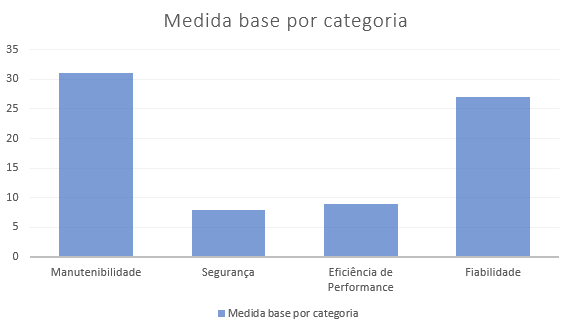
\includegraphics[width=0.7\linewidth]{graph_results_product.PNG}
	\caption{Número de regras violadas em função da característica de qualidade \small}
	\label{fig_quality}
\end{figure}

Com base no conhecimento que o grupo possui à cerca da equipa e do projeto em questão, este acredita que pode ser possível relacionar a natureza e particularidades de algumas das regras violadas com a falta de experiência da equipa de desenvolvido quanto a algumas das particularidades da arquitetura de software, uma vez que foi o maior e mais complexo projeto desenvolvido até ao momento da sua elaboração. Apesar de não existirem dados que permitam afirmar tal observação, as características de manutenibilidade e fiabilidade costumam de uma forma geral estar fortemente relacionadas com a experiência da equipa responsável pela conceção da solução, corroborando a hipótese. \\
Contudo, comparando os resultados das categorias de manutenibilidade e fiabilidade com as categorias de segurança e eficiência de performance é possível observar que houve um maior cuidado com estas duas últimas características. Considerando o contexto em que o projeto foi desenvolvido acredita-se que os resultados obtidos nestas duas categorias são fruto do cuidado com da cultura de testes utilizada nos projetos da Licenciatura assim como dos exemplos e práticas lecionadas nas Unidades Curriculares do 2º ano da Licenciatura, em especial Estruturas de Informação e Engenharia de Aplicações.

\section{Conclusões}
Relativamente à análise da qualidade do produto, as nossas observações permitem-nos concluir que estamos perante um produto que, à partida, é seguro e performante. Ainda assim, o produto em análise possui um número elevado de defeitos no que toca a boas práticas que promovem a manutenibilidade e fiabilidade, podendo comprometer a continuação do projeto de forma sustentável a nível de recursos e complexidade. \\
Baseando-se nos resultados descritos neste documento, o grupo reconhece que este tipo de análises são uma mais valia para avaliar de uma forma palpável os elementos do processo de desenvolvimento de software que devem ser melhorados num projeto assim como para avaliar quais as características cruciais que devem ser reavaliadas para a entrega de um produto de qualidade. O grupo reconhece também a importância e a mais valia das Unidades Curriculares de Laboratório/Projeto pois estas permitem desde cedo aos alunos ter um contacto com os aspetos chave do processo de desenvolvimento de software, ainda que de uma forma que pode ser considerada insatisfatória pelos padrões de qualidade utilizados na análise.

% -------------- BIBLIOGRAFIA -------------
\renewcommand\bibname{Referências} % mudar nome capítulo 
\addcontentsline{toc}{chapter}{Referências}
\setlength{\parskip}{0.7em}
\bibliographystyle{IEEEtran}
\bibliography{biblist.bib}

% --------------- ANEXOS -----------------
\begin{appendix}

\section*{Anexos}\label{ConteudoAnexos}

\subsection{Anexo 1 - Questionário Qualidade de Processo}\label{anexo_processo}
\begin{table}[H]
	\textbf{Gestão de Configuração}
		\centering
		\caption{Questionário 1 - Processo - Parte 1}
		\begin{tabular}{|p{5in}p{1in}|}		\hline
			\textbf{Questão}  & \textbf{Avaliação}\\ \hline
			1 - São identificados os itens de configuração, componentes e produtos de trabalho a serem 
	colocados sob a gestão de configuração?
	 & TI | \underline{\underline{\textbf{IP}}} | NI | NS \\ \hline
			2 - É estabelecido e mantido um sistema de gestão de configurações e gestão de alterações para 
	controlar os produtos de trabalho?
	 & TI | IP | \underline{\textbf{NI}} | NS \\ \hline
			3 -  São criados ou lançados baselines para uso interno e para entrega ao cliente?
	 & TI | \underline{\textbf{IP}} | NI | NS \\ \hline
			4 - Os pedidos de alterações dos itens de configuração são acompanhados?
	 & TI | \underline{\textbf{IP}} | NI | NS \\ \hline
			5 – As alterações nos itens de configuração são controladas?
	  & TI | IP | \underline{\textbf{NI}} | NS \\ \hline
			6 – São estabelecidos e mantidos registos de gestão de configurações que descrevem os itens 
	de configuração?
	 & TI | IP | \underline{\textbf{NI}} | NS \\ \hline
			7– Auditorias de configuração são realizadas para manter a integridade dos baselines?
	 & TI | IP | \underline{\textbf{NI}} | NS \\ \hline
		\end{tabular} 
	\end{table}
	
	%\begin{samepage}
		\begin{table}[H]
			\textbf{Medição e Análise}
				\centering
				\caption{Questionário 1 - Processo - Parte 2}
				\begin{tabular}{|p{5in}p{1in}|} \hline
					\textbf{Questão}  & \textbf{Avaliação}\\  \hline
					8 – São estabelecidos objetivos de medição?
			 & TI | IP | \underline{\textbf{NI}} | NS \\
					\hline
					9 – As medidas para satisfazer os objetivos de medição estão especificadas?
			 & TI | IP | \underline{\textbf{NI}} | NS \\
					\hline
					10 – Existe uma especificação de como os dados de medição são obtidos e armazenados - 
			(coleção de dados e respetivos procedimentos de armazenamento)?
			 & TI | IP | \underline{\textbf{NI}} | NS \\
					\hline
					11 – Existe uma especificação de como os dados de medição são análise) e comunicados?
			 & TI | IP | \underline{\textbf{NI}} | NS \\
					\hline
					12 – Os dados de medição especificados são obtidos?
			  & TI | IP | \underline{\textbf{NI}} | NS \\
					\hline
					13 – São analisados e interpretados os dados resultantes da medição?
			 & TI | IP | \underline{\textbf{NI}} | NS \\
					\hline
					14 – São geridos e armazenados os dados e resultados das medições, especificações de medição 
			e resultados da análise efetuada?
			 & TI | IP | \underline{\textbf{NI}} | NS \\
					\hline
					15 – Os resultados da medição e análise de atividades são comunicados a todas as partes
			interessadas?
			 & TI | IP | \underline{\textbf{NI}} | NS \\
					\hline
				\end{tabular} 
			\end{table}
			
			
	%\end{samepage}
	
	\begin{table}[H]
		\textbf{Monitorização e Controlo do Projeto}
			\centering
			\caption{Questionário 1 - Processo - Parte 3}
			\begin{tabular}{|p{5in}p{1in}|}		\hline
				\textbf{Questão}  & \textbf{Avaliação}\\ 
				\hline
				16 – São monitorizados os valores reais dos parâmetros do planeamento do projeto em relação 
		ao plano de projeto? 
		 & TI | \underline{\textbf{IP}} | NI | NS \\
				\hline
				17 – São monitorizados os compromissos em relação aos identificados no plano de projeto?
		 & TI | \underline{\textbf{IP}} | NI | NS \\
				\hline
				18 – São Monitorizados os riscos em relação aos identificados no plano do projeto?
		 & TI | \underline{\textbf{IP}} | NI | NS \\
				\hline
				19 – É monitorizada a gestão de dados do projeto em relação ao plano de projeto?
		 & TI | IP | \underline{\textbf{NI}} | NS \\
				\hline
				20 – É monitorizado o envolvimento das partes interessadas em relação ao plano de projeto?
		  & TI | IP | \underline{\textbf{NI}} | NS \\
				\hline
				21 – São revistos periodicamente o progresso, desempenho e as questões críticas do projeto?
		 & TI | \underline{\textbf{IP}} | NI | NS \\
				\hline
				22 – São revistos em pontos-chave selecionados do projeto, as realizações do projeto e os 
		resultados obtidos?
		 & \underline{\textbf{TI}} | IP | NI | NS \\
				\hline
				23 – São identificadas e analisadas as questões críticas e determinadas as ações corretivas 
		necessárias para tratar as mesmas?
		 & TI | \underline{\textbf{IP}} | NI | NS \\
				\hline
				24 – São implementadas ações corretivas para tratar as questões críticas identificadas?
		 & TI | \underline{\textbf{IP}} | NI | NS \\
				\hline
				25 – As ações corretivas são geridas até à sua conclusão?
		 & TI | \underline{\textbf{IP}} | NI | NS \\ \hline
			\end{tabular} 
		\end{table}
	
\begin{samepage}
	\begin{table}[H]
		\centering
		\textbf{Planeamento de Projeto}
		\caption{Questionário 1 - Processo - Parte 4}
			\begin{tabular}{|p{5in}p{1in}|}		
				\hline
				\textbf{Questão}  & \textbf{Avaliação}\\ 
				\hline
				26 – É estabelecida uma estrutura analítica de projeto (WBS) de alto nível para estimar o âmbito 
		do projeto?
		 & TI | IP | \underline{\textbf{NI}} | NS \\
				\hline
				27 – São estabelecidas e mantidas estimativas para atributos de produtos de trabalho e de 
		tarefas?
		 & TI | \underline{\textbf{IP}} | NI | NS \\
				\hline
				28 – As fases do ciclo de vida do projeto são definidas?
		 & \underline{\textbf{TI}} | IP | NI | NS \\
				\hline
				29 – As estimativas de esforço e de custo com base no raciocínio de estimativas são 
		determinadas?
		 & TI | \underline{\textbf{IP}} | NI | NS \\
				\hline
				30 – É estabelecido e mantido o orçamento e cronograma do projeto?
		  & TI | IP | \underline{\textbf{NI}} | NS \\
				\hline
				31 – São identificados e analisados os riscos do projeto?
		 & TI | IP | \underline{\textbf{NI}} | NS \\
				\hline
				32 – A gestão de dados do projeto é planeada?
		 & TI | IP | \underline{\textbf{NI}} | NS \\
				\hline
				33 – Os recursos necessários para a execução do projeto são planeados?
		 & TI | IP | \underline{\textbf{NI}} | NS \\
				\hline
				 34 – Os conhecimentos necessários para a execução do projeto são planeados?
				 & TI | \underline{\textbf{IP}} | NI | NS \\
				 \hline
				 35 – É planeado o envolvimento das partes interessadas identificadas?
				 & TI | IP | \underline{\textbf{NI}} | NS \\
				 \hline
				 36 – É estabelecido e mantido o plano global do projeto?
				 & TI | \underline{\textbf{IP}} | NI | NS \\
				 \hline
				 37 – Todos os planos que afetam o projeto para entender os compromissos do mesmo são 
		revistos?
				 & TI | IP | \underline{\textbf{NI}} | NS \\
				 \hline
				 38 – É ajustado o plano de projeto de acordo com os recursos estimados e disponíveis?
				 & TI | \underline{\textbf{IP}} | NI | NS \\
				 \hline
				39 – O compromisso das partes interessadas relevantes, responsáveis pela execução e apoio à 
		execução do plano é obtido?
				 & TI | IP | \underline{\textbf{NI}} | NS \\
				\hline

		\end{tabular}		
	\end{table}	
		\end{samepage}
	
	
	\begin{table}[H]
	\textbf{Garantia da Qualidade de Processo e Produto}
		\centering
		\caption{Questionário 1 - Processo - Parte 5}
		\begin{tabular}{|p{5in}p{1in}|}		
			\hline
			\textbf{Questão}  & \textbf{Avaliação}\\ 
			\hline
			40 – São avaliados objetivamente os processos selecionados em relação às descrições de 
	processo, padrões e procedimentos aplicáveis?
	 & TI | IP | \underline{\textbf{NI}} | NS \\
			\hline
			41 – São avaliados objetivamente os produtos de trabalho selecionados em relação às descrições 
	de processo, padrões e procedimentos aplicáveis?
	 & TI | \underline{\textbf{IP}} | NI | NS \\
			\hline
			42 – São comunicadas as questões críticas relativas à qualidade e asseguradas a resolução de 
	não conformidades com a equipa e os gestores?
	 & TI | IP | \underline{\textbf{NI}} | NS \\
			\hline
			43 – Os registos das atividades de garantia da qualidade são estabelecidos e mantidos?
	 & TI | IP | \underline{\textbf{NI}} | NS \\
			\hline
		\end{tabular} 
	\end{table}
	
	\begin{table}[H]
	\textbf{Gestão de Requisitos}
		\centering
		\caption{Questionário 1 - Processo - Parte 6}
		\begin{tabular}{|p{5in}p{1in}|}		
			\hline
			\textbf{Questão}  & \textbf{Avaliação}\\ 
			\hline
			44 – É realizado um trabalho em conjunto, com quem definiu os requisitos de forma a obter um 
	melhor entendimento do significado dos mesmos?
	 & \underline{\textbf{TI}} | IP | NI | NS \\
			\hline
			45 – É obtido o compromisso com os participantes do projeto face aos requisitos?
	 & \underline{\textbf{TI}} | IP | NI | NS \\
			\hline
			46 – As mudanças nos requisitos à medida que evoluem durante o projeto são geridas?
	 & TI | \underline{\textbf{TI}} | NI | NS \\
			\hline
			47 – É mantida a rastreabilidade bidirecional dos requisitos e produtos de trabalho?
	 & TI | \underline{\textbf{TI}} | NI | NS \\
			\hline
			48 – É garantido que os planos de projeto e produtos de trabalho permanecem alinhados com 
	as exigências?
	  & TI | IP | \underline{\textbf{NI}} | NS \\
			\hline
		\end{tabular} 
	\end{table}
	
	\begin{table}[H]
	\textbf{Gestão de Contrato com Fornecedores}
		\centering
		\caption{Questionário 1 - Processo - Parte 7}
		\begin{tabular}{|p{5in}p{1in}|}		
			\hline
			\textbf{Questão}  & \textbf{Avaliação}\\ 
			\hline
			49 – É determinado o tipo de aquisição para cada produto ou componente de produto a ser 
	adquirido?
	 & TI | IP | NI | \underline{\textbf{NS}} \\
			\hline
			50 – Os fornecedores são selecionados com base numa avaliação da sua capacidade em 
	satisfazer os requisitos especificados e critérios estabelecidos?
	 & TI | IP | NI | \underline{\textbf{NS}} \\
			\hline
			51 – São estabelecidos e mantidos contractos formais com os fornecedores?
	 & TI | IP | NI | \underline{\textbf{NS}} \\
			\hline
			52 – São executadas atividades com o fornecedor conforme especificado no contrato com o 
	mesmo?
	 & TI | IP | NI | \underline{\textbf{NS}} \\
			\hline
			53 – Existe a verificação que o acordo com o fornecedor está satisfeito, antes de aceitar o 
	produto adquirido?
	  & TI | IP | NI | \underline{\textbf{NS}} \\
			\hline
			54 – É assegurada a transição dos produtos adquiridos no fornecedor?
	 & TI | IP | NI | \underline{\textbf{NS}} \\
			\hline
		\end{tabular} 
	\end{table}
	
	\begin{table}[H]
	\textbf{Análise e Tomada de Decisões}
		\centering
		\caption{Questionário 1 - Processo - Parte 8}
		\begin{tabular}{|p{5in}p{1in}|}		
			\hline
			\textbf{Questão}  & \textbf{Avaliação}\\ 
			\hline
			55 – São estabelecidas e mantidas diretrizes para determinar quais as questões que são sujeitas 
	a um processo formal?
	 & TI | IP | NI | \underline{\textbf{NS}} \\
			\hline
			56 – São estabelecidos e mantidos critérios para avaliar as alternativas e para classificá-los de 
	forma relativa?
	 & TI | IP | \underline{\textbf{NI}} | NS \\
			\hline
			57 – As soluções alternativas para resolver problemas são identificadas?
	 & TI | \underline{\textbf{IP}} | NI | NS \\
			\hline
			58 – São selecionados métodos de avaliação?
	 & TI | IP | \underline{\textbf{NI}} | NS \\
			\hline
			59 – As soluções alternativas usando critérios e métodos estabelecidos são avaliadas?
	  & TI | IP | \underline{\textbf{NI}} | NS \\
			\hline
			60 – São selecionadas soluções a partir das várias alternativas, com base nos critérios de 
	avaliação?
	 & TI | IP | \underline{\textbf{NI}} | NS \\
			\hline
		\end{tabular} 
	\end{table}
	
	\begin{table}[H]
	\textbf{Gestão Integrada do Projeto}
		\centering
		\caption{Questionário 1 - Processo - Parte 9}
		\begin{tabular}{|p{5in}p{1in}|}		
			\hline
			\textbf{Questão}  & \textbf{Avaliação}\\ 
			\hline
			61 – É estabelecido e mantido o processo definido para o projeto desde o início até ao fim do mesmo?
	 & TI | \underline{\textbf{IP}} | NI | NS \\
			\hline
			62 – São utilizados os ativos do processo e o repositório de medições da organização para 
	estimar e planear as atividades do projeto?
	 & TI | \underline{\textbf{IP}} | NI | NS \\
			\hline
			63 – É estabelecido e mantido o ambiente de trabalho do projeto com base nos padrões de 
	ambiente de trabalho da organização?
	 & TI | \underline{\textbf{IP}} | NI | NS \\
			\hline
			64 – É integrado o plano do projeto e outros planos que afetam o projeto para descrever o 
	processo definido do mesmo?
	 & TI | IP | \underline{\textbf{NI}} | NS \\
			\hline
			65 – O projeto é gerido usando o plano de projeto, outros planos que afetam o projeto e o 
	processo definido para o mesmo?
	  & TI | IP | \underline{\textbf{NI}} | NS \\
			\hline
			66 – As equipas de projeto são estabelecidas e mantidas?
	 & \underline{\textbf{TI}} | IP | NI | NS \\
			\hline
			67 – Existe a contribuição de experiências do processo relacionado com os processos ativos da 
	organização?
	 & TI | \underline{\textbf{IP}} | NI | NS \\
			\hline
			68 – É feita a gestão do envolvimento das partes interessadas?
	 & TI | IP | \underline{\textbf{NI}} | NS \\
			\hline
			69  – Existe a colaboração com as partes interessadas na identificação, negociação e 
	acompanhamento de dependências críticas?
	 & TI | IP | \underline{\textbf{NI}} | NS \\
			\hline
			70 – São resolvidas questões críticas de coordenação com as partes interessadas?
	 & TI | IP | \underline{\textbf{NI}} | NS \\
			\hline
		\end{tabular} 
	\end{table}
	
	\begin{table}[H]
	\textbf{Definição dos Processos da Organização}
		\centering
		\caption{Questionário 1 - Processo - Parte 10}
		\begin{tabular}{|p{5in}p{1in}|}		
			\hline
			\textbf{Questão}  & \textbf{Avaliação}\\ 
			\hline
			71 – São estabelecidos e mantidos processos-padrão da organização?
	 & TI | \underline{\textbf{IP}} | NI | NS \\
			\hline
			72 – As descrições dos modelos do ciclo de vida aprovados para uso da organização são 
	estabelecidas e mantidas?
	 & TI | \underline{\textbf{IP}} | NI | NS \\
			\hline
			73 – Critérios e diretrizes para adaptação do conjunto de processos-padrão da organização são 
	estabelecidos e mantidos?
	 & TI | IP | \underline{\textbf{NI}} | NS \\
			\hline
			74 – O repositório de medições da organização é estabelecido e mantido?
	 & TI | IP | \underline{\textbf{NI}} | NS \\
			\hline
			75 – A biblioteca de processos ativos da organização é estabelecida e mantida?
	  & TI | IP | NI | \underline{\textbf{NS}} \\
			\hline
			76 – Os padrões de ambiente de trabalho são estabelecidos e mantidos?
	 & TI | \underline{\textbf{IP}} | NI | NS \\
			\hline
			77 – Regras de organização e diretrizes para a estrutura, formação e funcionamento das equipas 
	são estabelecidas e mantidas?
	& TI | \underline{\textbf{IP}} | NI | NS \\
			\hline
		\end{tabular} 
	\end{table}
	
	%\begin{table}[H]
		\centerline{\textbf{Enfoque nos Processos da Organização}}
		\begin{longtable}{|p{5in}p{1in}|}
			\caption{Questionário 1 - Processo - Parte 11}	
			\endhead	
			\hline
			\textbf{Questão}  & \textbf{Avaliação}\\ 
			\hline
			78 – A descrição das necessidades e objetivos dos processos da organização são estabelecidos e 
	mantidos?
	 & TI | \underline{\textbf{IP}} | NI | NS \\
			\hline
			79 – São avaliados periodicamente os processos da organização e conforme necessário, para 
	conhecer os seus pontos fortes e fracos?
	 & TI | IP | \underline{\textbf{NI}} | NS \\
			\hline
			80 – As melhorias para os processos da organização e ativos do processo são identificadas?
	 & TI | IP | \underline{\textbf{NI}} | NS \\
			\hline
			81 – São estabelecidos e mantidos planos de ações do processo para promover melhorias nos 
	processos e ativos de processo?
	 & TI | IP | NI | \underline{\textbf{NS}} \\
			\hline
			82 – Os planos de ações de processo são implementados?
	  & TI | IP | NI | \underline{\textbf{NS}} \\
			\hline
			83 – Os ativos de processos organizações são implantados em toda a organização?
	 & TI | IP | NI | \underline{\textbf{NS}} \\
			\hline
			84 – O conjunto de processos-padrão são implantados nos projetos desde o início do mesmo, e 
	a implementação de mudanças nesses processos ao longo do ciclo de vida de cada projeto
	conforme apropriado são igualmente tornados comuns? 
	 & TI | IP | NI | \underline{\textbf{NS}} \\
	 \hline
			85 – A implementação do conjunto de processos-padrão da organização e o uso de ativos de
	processos em todos os projetos é monitorizada? 
	 & TI | IP | NI | \underline{\textbf{NS}} \\
	 \hline
			86 – São incorporadas experiências em ativos de processos organizacionais?
	 & TI | IP | NI | \underline{\textbf{NS}} \\
			\hline
		\end{longtable}
	%\end{table}
	
	\begin{table}[H]
	\textbf{Formação na Organização}
		\centering
		\caption{Questionário 1 - Processo - Parte 12}
		\begin{tabular}{|p{5in}p{1in}|}		
			\hline
			\textbf{Questão}  & \textbf{Avaliação}\\ 
			\hline
			87 – As necessidades de formação estratégicas da organização são estabelecidas e mantidas?
	 & TI | IP | NI | \underline{\textbf{NS}} \\
			\hline
			88 – São determinadas quais as necessidades de formação são da responsabilidade da 
	organização e quais devem ser atribuídas a projetos individuais ou grupos de trabalho?
	 & TI | \underline{\textbf{IP}} | NI | NS \\
			\hline
			89 – Um plano tático de formação da organização é estabelecido e mantido?
	 & TI | \underline{\textbf{IP}} | NI | NS \\
			\hline
			90 – A capacidade de formação para tratar das necessidades de formação na organização é 
	estabelecida e mantida?
	 & TI | \underline{\textbf{IP}} | NI | NS \\
			\hline
			91 – É fornecida formação de acordo com o plano tático de formação da organização?
	  & TI | \underline{\textbf{IP}} | NI | NS \\
			\hline
			92 – Registos de formação da organização são estabelecidos e mantidos?
	 & TI | \underline{\textbf{IP}} | NI | NS \\
	 \hline
			93 – A eficácia do programa de formação da organização é avaliada?
	 & TI | \underline{\textbf{IP}} | NI | NS \\
			\hline
		\end{tabular} 
	\end{table}
	
	\begin{table}[h]
	\textbf{Integração de Produto}
		\centering
		\caption{Questionário 1 - Processo - Parte 13}
		\begin{tabular}{|p{5in}p{1in}|}		
			\hline
			\textbf{Questão}  & \textbf{Avaliação}\\ 
			\hline
			94 – Uma estratégia de integração de produto é estabelecida e mantida?
	 & TI | \underline{\textbf{IP}} | NI | NS \\
			\hline
			95 – O ambiente necessário para apoiar a integração dos componentes de produto é 
	estabelecido e mantido?
	 & TI | \underline{\textbf{IP}} | NI | NS \\
			\hline
			96 – Procedimentos e critérios para a integração dos componentes de produto são estabelecidos 
	e mantidos?
	 & TI | \underline{\textbf{IP}} | NI | NS \\
			\hline
			97 – São revistas as descrições de interface de forma a assegurar a cobertura e completude da 
	mesma?
	 & TI | IP | \underline{\textbf{NI}} | NS \\
			\hline
			98 – São geridas as definições de interfaces internos e externos, designs e mudanças de produtos 
	e componentes de produto?
	  & TI | \underline{\textbf{IP}} | NI | NS \\
			\hline
			99 – É confirmado se os componentes de produto estão prontos a serem integrados de acordo 
	com a descrição, e as interfaces dos componentes de produto estão em conformidade com as
	respetivas descrições? 
	 & TI | IP | \underline{\textbf{NI}} | NS \\
	 \hline
			100 – A integração e montagem dos componentes de produto estão de acordo com a estratégia
	de integração do produto e procedimentos disponíveis? 
	 & TI | IP | \underline{\textbf{NI}} | NS \\
	 \hline
			101 – Existe a avaliação dos componentes de produto integrado e compatibilidade com as
	interfaces? 
	 & TI | IP | \underline{\textbf{NI}} | NS \\
	 \hline
			102 – O produto integrado ou o componente do produto é transformado em package e é
	entregue ao cliente? 
	 & TI | \underline{\textbf{IP}} | NI | NS \\
			\hline
		\end{tabular} 
	\end{table}
	
	%\begin{table}[h]
	\centerline{\textbf{Desenvolvimento de Requisitos}}
		%\centering		
		\begin{longtable}{|p{5in}p{1in}|}
			\caption{Questionário 1 - Processo - Parte 14}
			\endhead		
			\hline
			\textbf{Questão}  & \textbf{Avaliação}\\ 
			\hline
			103 – O levantamento das necessidades, expectativas, restrições e interfaces para todas as fases 
	do ciclo de vida do produto é efetuado?
	 & TI | IP | \underline{\textbf{NI}} | NS \\
			\hline
			104 – As necessidades, expectativas, restrições e interfaces são transformados em requisitos 
	prioritários do cliente?
	 & TI | \underline{\textbf{IP}} | NI | NS \\
			\hline
			105 – Os requisitos de produto e de componente de produto, com base nas necessidades do 
	cliente são estabelecidos e mantidos?
	 & TI | \underline{\textbf{IP}} | NI | NS \\
			\hline
			106 – Os requisitos de cada componente de produto são atribuídos?
	 & TI | \underline{\textbf{IP}} | NI | NS \\
			\hline
			107 – Os requisitos de interface são identificados?
	  & TI | \underline{\textbf{IP}} | NI | NS \\
			\hline
			108 – Conceitos operacionais e cenários associados são estabelecidos e mantidos?
	 & TI | \underline{\textbf{IP}} | NI | NS \\
	 \hline
			109 – Uma definição de funcionalidade e atributos de qualidade é estabelecida e mantida?
	 & TI | IP | NI | \underline{\textbf{NS}} \\
	 \hline
		110 – Os requisitos para assegurar que são necessários e suficientes são analisados?
	 & TI | IP | \underline{\textbf{NI}} | NS \\
	 \hline
			111 – Os requisitos para equilibrar as necessidades e as restrições das partes interessadas são 
	analisados?
	 & TI | IP | \underline{\textbf{IP}} | NS \\
			\hline
			112 – Os requisitos para assegurar que o produto final irá funcionar conforme o esperado no 
	ambiente do utilizador final são validados?
	 & TI | \underline{\textbf{IP}} | NI | NS \\
			\hline
		%\end{tabular} 
	\end{longtable}
	
	\begin{table}[H]
	\textbf{Gestão de Risco}
		\centering
		\caption{Questionário 1 - Processo - Parte 15}
		\begin{tabular}{|p{5in}p{1in}|}		
			\hline
			\textbf{Questão}  & \textbf{Avaliação}\\ 
			\hline
			113 – Fontes e categorias de riscos são definidos?
	 & TI | IP | \underline{\textbf{NI}} | NS \\
			\hline
			114 – Os parâmetros utilizados para analisar e categorizar os riscos e controlar o esforço de 
	gestão de riscos são definidos?
	 & TI | IP | \underline{\textbf{NI}} | NS \\
			\hline
			115 – Uma estratégia a ser utilizada para a gestão de riscos é estabelecida e mantida?
	 & TI | IP | \underline{\textbf{NI}} | NS \\
			\hline
			116 – A identificação e documentação dos riscos é feita?
	 & TI | IP | \underline{\textbf{NI}} | NS \\
			\hline
		117 – É avaliado e classificado cada risco identificado, utilizando as categorias e os parâmetros 
	definidos para os riscos e determinada a sua prioridade relativa?
	  & TI | IP | \underline{\textbf{NI}} | NS \\
			\hline
			118 – Um plano de atenuação de risco de acordo com a estratégia de gestão de riscos é 
	desenvolvido?
	 & TI | IP | \underline{\textbf{NI}} | NS \\
	 \hline
			119 – É Monitorizado periodicamente o status de cada risco, e implementado o plano de 
	atenuação de risco quando necessário?
	 & TI | IP | \underline{\textbf{NI}} | NS \\
			\hline
		\end{tabular} 
	\end{table}
	
	\begin{table}[H]
	\textbf{Solução Técnica}
	\centering
		\caption{Questionário 1 - Processo - Parte 16}
		\begin{tabular}{|p{5in}p{1in}|}		
			\hline
			\textbf{Questão}  & \textbf{Avaliação}\\ 
			\hline
			120 – Soluções alternativas e critérios de seleção são desenvolvidos?
	 & TI | IP | \underline{\textbf{NI}} | NS \\
			\hline
			121 – São selecionadas as soluções associadas a componentes de produto baseadas em critérios 
	de seleção?
	 & TI | IP | \underline{\textbf{NI}} | NS \\
			\hline
			122 – Um design para o produto ou componente de produto é desenvolvido?
	 & TI | \underline{\textbf{NI}} | NI | NS \\
			\hline
			123 – Um pacote de dados técnicos é estabelecido e mantido?
	 & TI | IP | \underline{\textbf{NI}} | NS \\
			\hline
			124 – Projetar as interfaces dos componentes de produto usando critérios estabelecidos é 
	realizado? 
	  & TI | IP | \underline{\textbf{NI}} | NS \\
			\hline
			125 – É avaliado se os componentes de produto devem ser desenvolvidos, comprados ou 
	reutilizados com base em critérios estabelecidos? 
	 & TI | IP | \underline{\textbf{NI}} | NS \\
	 \hline
			126 – O design dos componentes de produto é implementado?
	 & TI | \underline{\textbf{NI}} | NI | NS \\
			\hline
			127 – A elaboração e atualização da documentação para o utilizador final são realizadas?
	 & TI | \underline{\textbf{NI}} | NI | NS \\
			\hline
		\end{tabular} 
	\end{table}
	
	\begin{table}[H]
	\textbf{Validação}
		\centering
		\caption{Questionário 1 - Processo - Parte 17}
		\begin{tabular}{|p{5in}p{1in}|}		
			\hline
			\textbf{Questão}  & \textbf{Avaliação}\\ 
			\hline
			128 – São selecionados os produtos ou componentes de produto a serem validados e os 
	métodos de validação a serem utilizados?
	 & TI | \underline{\textbf{IP}} | NI | NS \\
			\hline
			129 – O ambiente necessário para suportar a validação é estabelecido e mantido?
	 & TI | \underline{\textbf{IP}} | NI | NS \\
			\hline
			130 – Os procedimentos e critérios de validação são estabelecidos e mantidos?
	 & TI | IP | \underline{\textbf{NI}} | NS \\
			\hline
			131 – É realizada a validação dos produtos e componentes de produto selecionados?
	 & TI | \underline{\textbf{IP}} | NI | NS \\
			\hline
			132 – Os resultados das atividades de validação são analisados?
	  & TI | \underline{\textbf{IP}} | NI | NS \\
			\hline
		\end{tabular} 
	\end{table}
	
	\begin{table}[H]
	\textbf{Verificação }
		\centering
		\caption{Questionário 1 - Processo - Parte 18}
		\begin{tabular}{|p{5in}p{1in}|}		
			\hline
			\textbf{Questão}  & \textbf{Avaliação}\\ 
			\hline
			133 – Os produtos de trabalho a serem verificados e os métodos de verificação a serem 
	utilizados são selecionados?
	 & TI | \underline{\textbf{IP}} | NI | NS \\
			\hline
			134 – O ambiente necessário para suportar a verificação é estabelecido e mantido?
	 & TI | \underline{\textbf{IP}} | NI | NS \\
			\hline
			135 – Os procedimentos e critérios de verificação para os produtos de trabalho selecionados são 
	estabelecidos e mantidos?
	 & TI | \underline{\textbf{IP}} | NI | NS \\
			\hline
			136 – Existe preparação para a revisão por pares dos produtos de trabalho selecionados?
	 & TI | IP | \underline{\textbf{NI}} | NS \\
			\hline
			137 – É realizada a revisão por pares nos produtos de trabalho selecionados e identificados 
	problemas resultantes da revisão efetuada?
	  & TI | IP | \underline{\textbf{NI}} | NS \\
			\hline
			138 – Os dados sobre a preparação, realização e resultados obtidos destas revisões são 
	analisados?
	 & TI | IP | \underline{\textbf{NI}} | NS \\
	 \hline
			139 – A verificação nos produtos de trabalho selecionados é realizada?
	 & TI | \underline{\textbf{IP}} | NI | NS \\
	  \hline
			140 – Os resultados de todas as atividades de verificação são analisados? 
	 & TI | IP | \underline{\textbf{NI}} | NS \\
			\hline
		\end{tabular} 
	\end{table}
	
\subsection{Anexo 2 - Critérios de Classificação (Práticas, Metas e Áreas de Processo)}\label{anexo_processo_classificacao}

\begin{table}[H]
	\textbf{Classificação - Prática}
		\centering
		\caption{Critérios de Classificação - Prática}
		\begin{tabular}{|p{1in}p{5in}|}		
			\hline
			\textbf{Classificação}  & \textbf{Critérios}\\ 
			\hline
			Totalmente implementada	(TI) & Quando a prática está bem estabelecida e é executada de forma
			consistente e sempre \\
			\hline
			Implementada em parte (IP) & Quando a prática está bem estabelecida e é geralmente executada
			(quase sempre) \\
			\hline
			Não implementada (IP/NI) & Prática está estabelecida, mas é executada apenas algumas vezes; ou
			Quando não é executada em nenhuma circunstância; \\
			\hline
			Não sei (NS) & Quando o inquirido não sabe responder/desconhece se a prática está
			implementada \\
			\hline
		\end{tabular} 
\end{table}

\begin{table}[H]
	\textbf{Classificação - Meta}
		\centering
		\caption{Critérios de Classificação - Meta}
		\begin{tabular}{|p{1in}p{5in}|}		
			\hline
			\textbf{Classificação}  & \textbf{Critérios}\\ 
			\hline
			Não avaliada (NAv) & Práticas associadas não estão avaliadas (NS) ou classificadas como NA;
			Os dados existentes não são suficientes para classificar a meta \\
			\hline
			Satisfeita (Sat) & Se ambas as condições forem verdadeiras:
			• A maioria das práticas estão classificadas como TI e as restantes,
			se existirem, parcialmente;
			• A agregação das fraquezas associadas à meta não tem um impacto
			negativo na realização da meta.	 \\
			\hline
			Não satisfeita (NSat) & Necessário descrever a forma como o conjunto de pontos negativos
			(ou apenas um) levaram a essa classificação. \\
			\hline
		\end{tabular} 
\end{table}

\begin{table}[H]
	\textbf{Classificação - Área de Processo}
		\centering
		\caption{Critérios de Classificação - Área de Processo}
		\begin{tabular}{|p{1in}p{5in}|}		
			\hline
			\textbf{Classificação}  & \textbf{Critérios}\\ 
			\hline
			Não avaliada (NAv) & Uma das metas classificada como não avaliada (NAv) e nenhuma das
			outras classificadas como não satisfeita (NSat) \\
			\hline
			Satisfeita (Sat) & Todas as metas da área classificadas como satisfeitas (Sat);
			Caso exista alguma classificada como não satisfeita (NSat) não poderá
			ter impacto negativo na realização da área \\
			\hline
			Não satisfeita (NSat) & Todas as metas da área classificadas como não satisfeitas (NSat); ou
			Uma das metas consideradas importantes classificada como não
			satisfeita (NSat) \\
			\hline
			Não Aplicável(NAp) & Área de processo determinada como não aplicável à Organização, ou
			fora do âmbito do modelo \\
			\hline
		\end{tabular} 
\end{table}

\subsection{Anexo 3 - Questionário Qualidade de Produto}
\label{anexo_produto}
De modo a analisar a avaliar a qualidade do produto, em foi desenvolvido o seguinte questionário que se encontra dividido em quatro grupos, representando medidas padrão: Manutenibilidade, Segurança, Eficiência da Performance e Fiabilidade.
Cada grupo, que representa uma caraterística a ser avaliada, contém um conjunto de regras de qualidade, para o qual terá de ser indicado o número de violações da mesma.

Grupo 1: Manutenibilidade
O propósito destas regras é estabelecer uma medida padrão de manutenibilidade com base na deteção de violações de boas práticas arquiteturais e de codificação que podem resultar em operações não confiáveis, como interrupções, corrupção de dados e longa recuperação de falhas do sistema.
\begin{samepage}
\begin{itemize}
	\setlength\itemsep{0em}
	\item ASCMM-MNT-1: Control Flow Transfer Control Element outside Switch Block
	\item ASCMM-MNT-2: Class Element Excessive Inheritance of Class Elements with Concrete Implementation
	\item ASCMM-MNT-3: Storable and Member Data Element Initialization with Hard-Coded Literals
	\item ASCMM-MNT-4: Callable and Method Control Element Number of Outward Calls
	\item ASCMM-MNT-5: Loop Value Update within the Loop
	\item ASCMM-MNT-6: Commented-out Code Element Excessive Volume
	\item ASCMM-MNT-7: Inter-Module Dependency Cycles
	\item ASCMM-MNT-8: Source Element Excessive Size
	\item ASCMM-MNT-9: Horizontal Layer Excessive Number
	\item ASCMM-MNT-10: Named Callable and Method Control Element Multi-Layer Span
	\item ASCMM-MNT-11: Callable and Method Control Element Excessive Cyclomatic Complexity Value
	\item ASCMM-MNT-12: Named Callable and Method Control Element with Layer-skipping Call
	\item ASCMM-MNT-13: Callable and Method Control Element Excessive Number of Parameters
	\item ASCMM-MNT-14: Callable and Method Control Element Excessive Number of Control Elements involving Data Element from Data Manager or File Resource
	\item ASCMM-MNT-15: Public Member Element	
	\item ASCMM-MNT-16: Method Control Element Usage of Member Element from other Class Element
	\item ASCMM-MNT-17: Class Element Excessive Inheritance Level
	\item ASCMM-MNT-18: Class Element Excessive Number of Children
	\item ASCMM-MNT-19: Named Callable and Method Control Element Excessive Similarity
	\item ASCMM-MNT-20: Unreachable Named Callable or Method Control Element
\end{itemize}
\end{samepage}
Grupo 2: Segurança
O propósito destas regras é estabelecer uma medida padrão de segurança com base na deteção de violações de boas práticas arquiteturais e de codificação que poderão resultar na entrada não autorizada em sistemas, roubo de informações confidenciais, e o comprometimento malicioso da integridade do sistema.
\begin{itemize}
	\setlength\itemsep{0em}
	\item ASCSM-CWE-22: Path Traversal Improper Input Neutralization
	\item ASCSM-CWE-78: OS Command Injection Improper Input Neutralization
	\item ASCSM-CWE-79: Cross-site Scripting Improper Input Neutralization
	\item ASCSM-CWE-89: SQL Injection Improper Input Neutralization
	\item ASCSM-CWE-99: Name or Reference Resolution Improper Input Neutralization
	\item ASCSM-CWE-120: Buffer Copy without Checking Size of Input
	\item ASCSM-CWE-129: Array Index Improper Input Neutralization
	\item ASCSM-CWE-134: Format String Improper Input Neutralization
	\item ASCSM-CWE-252-resource: Unchecked Return Parameter Value of named Callable and Method Control Element with Read, Write, and Manage Access to Platform Resource
	\item ASCSM-CWE-327: Broken or Risky Cryptographic Algorithm Usage
	\item ASCSM-CWE-396: Declaration of Catch for Generic Exception
	\item ASCSM-CWE-397: Declaration of Throws for Generic Exception
	\item ASCSM-CWE-434: File Upload Improper Input Neutralization
	\item ASCSM-CWE-456: Storable and Member Data Element Missing Initialization
	\item ASCSM-CWE-606: Unchecked Input for Loop Condition
	\item ASCSM-CWE-667: Shared Resource Improper Locking
	\item ASCSM-CWE-672: Expired or Released Resource Usage
	\item ASCSM-CWE-681: Numeric Types Incorrect Conversion
	\item ASCSM-CWE-772: Missing Release of Resource after Effective Lifetime
	\item ASCSM-CWE-789: Uncontrolled Memory Allocation
	\item ASCSM-CWE-798: Hard-Coded Credentials Usage for Remote Authentication
	\item ASCSM-CWE-835: Loop with Unreachable Exit Condition ('Infinite Loop')
\end{itemize} 

Grupo 3: Eficiência de Performance
O propósito destas regras é estabelecer uma medida padrão de segurança com base na deteção de violações de boas práticas arquiteturais e de codificação que poderão resultar numa operação ineficiente, como a degradação do desempenho ou uso excessivo de recursos do processador.
\begin{itemize}	
\setlength\itemsep{0em}
	\item ASCPEM-PRF-1: Static Block Element containing Class Instance Creation Control Element
	\item ASCPEM-PRF-2: Immutable Storable and Member Data Element Creation
	\item ASCPEM-PRF-3: Static Member Data Element outside of a Singleton Class Element
	\item ASCPEM-PRF-4: Data Resource Read and Write Access Excessive Complexity
	\item ASCPEM-PRF-5: Data Resource Read Access Unsupported by Index Element
	\item ASCPEM-PRF-6: Large Data Resource ColumnSet Excessive Number of Index Elements
	\item ASCPEM-PRF-7: Large Data Resource ColumnSet with Index Element of Excessive Size
	\item ASCPEM-PRF-8: Control Elements Requiring Significant Resource Element within Control Flow Loop Block
	\item ASCPEM-PRF-9: Non-stored SQL Callable Control Element with Excessive Number of Data Resource Access
	\item ASCPEM-PRF-10: Non-SQL Named Callable and Method Control Element with Excessive Number of Data Resource Access
	\item ASCPEM-PRF-11: Data Access Control Element from Outside Designated Data Manager Component
	\item ASCPEM-PRF-12: Storable and Member Data Element Excessive Number of Aggregated Storable and Member Data Elements
	\item ASCPEM-PRF-13: Data Resource Access not using Connection Pooling Capability
	\item ASCPEM-PRF-14: Storable and Member Data Element Memory Allocation Missing De-allocation Control Element
	\item ASCPEM-PRF-15: Storable and Member Data Element Reference Missing De-referencing Control Element
\end{itemize}

Grupo 4: Fiabilidade
O propósito destas regras é estabelecer uma medida padrão de segurança com base na deteção de violações de boas práticas arquiteturais e de codificação que poderão resultar em operações não confiáveis, como interrupções, corrupção de dados e recuperação de falhas do sistema.
\begin{itemize}
	\setlength\itemsep{0em}
	\item ASCRM-CWE-252-data: Unchecked Return Parameter Value of named Callable and Method Control Element with Read, Write, and Manage Access to Data Resource
	\item ASCRM-CWE-252-resource: Unchecked Return Parameter Value of named Callable and Method Control Element with Read, Write, and Manage Access to Platform Resource
	\item ASCRM-CWE-396: Declaration of Catch for Generic Exception
	\item ASCRM-CWE-397: Declaration of Throws for Generic Exception
	\item ASCRM-CWE-456: Storable and Member Data Element Missing Initialization
	\item ASCRM-CWE-674: Uncontrolled Recursion
	\item ASCRM-CWE-704: Incorrect Type Conversion or Cast
	\item ASCRM-CWE-772: Missing Release of Resource after Effective Lifetime
	\item ASCRM-CWE-788: Memory Location Access After End of Buffer
	\item ASCRM-RLB-1: Empty Exception Block
	\item ASCRM-RLB-2: Serializable Storable Data Element without Serialization Control Element
	\item ASCRM-RLB-3: Serializable Storable Data Element with non-Serializable Item Elements
	\item ASCRM-RLB-4: Persistent Storable Data Element without Proper Comparison Control Element
	\item ASCRM-RLB-5: Runtime Resource Management Control Element in a Component Built to Run on Application Servers
	\item ASCRM-RLB-6: Storable or Member Data Element containing Pointer Item Element without Proper Copy Control Element
	\item ASCRM-RLB-7: Class Instance Self Destruction Control Element
	\item ASCRM-RLB-8: Named Callable and Method Control Elements with Variadic Parameter Element
	\item ASCRM-RLB-9: Float Type Storable and Member Data Element Comparison with Equality Operator
	\item ASCRM-RLB-10: Data Access Control Element from Outside Designated Data Manager Component
	\item ASCRM-RLB-11: Named Callable and Method Control Element in Multi-Thread Context with non-Final Static Storable or Member Element
	\item ASCRM-RLB-12: Singleton Class Instance Creation without Proper Lock Element Management
	\item ASCRM-RLB-13: Inter-Module Dependency Cycles
	\item ASCRM-RLB-14: Parent Class Element with References to Child Class Element
	\item ASCRM-RLB-15: Class Element with Virtual Method Element without Virtual Destructor
	\item ASCRM-RLB-16: Parent Class Element without Virtual Destructor Method Element
	\item ASCRM-RLB-17: Child Class Element without Virtual Destructor unlike its Parent Class Element
	\item ASCRM-RLB-18: Storable and Member Data Element Initialization with Hard-Coded Network Resource Configuration Data
	\item ASCRM-RLB-19: Synchronous Call Time-Out Absence
\end{itemize}






%\begin{figure}[h]
%	\centering
%	\includegraphics[width=0.4\linewidth]{}
%	\caption{Exemplo de imagem: \small{\textit{Fonte: 	\cite{CMMI2010}}}}
%	\label{fig:figura1}
%\end{figure}


\end{appendix}
\end{document}
